% Chapter Template

\chapter{Evaluation} % Main chapter title

\label{evaluation} % Change X to a consecutive number; for referencing this chapter elsewhere, use \ref{ChapterX}

In this chapter, the different machine learning algorithms are evaluated. In Section~\ref{datasets}, the different evaluation steps are explained. There are four steps. Step one is the training of the machine learning algorithm, this is evaluated using learning curves. Step two is evaluation within the same dataset, this is done using the CTU dataset.. In the third step, cross-dataset validation is done. The algorithms are evaluated by using multiple datasets containing real-world data. In the final step, unlabeled real-world data is used. \\
\\
For the first and second step, the algorithms are always trained using a subset from the datasets and tested using another subset. Since the datasets contain a lot of different labels (and thus classes), it has been chosen not to always follow the "30/70" rule as explained in Section~\ref{evaluationHypothesis}. Instead the algorithm is trained using the number of training samples that indicates a good accuracy in the learning curves, and tested using a set of $~230000$ samples. This number was found by looking at all the learning curves from the different algorithms and choose the appropriate training size. From these training sizes, the largest value was chosen and on this value the "30/70" rule was used. This was done to make sure that every experiment was tested using the same amount of samples and that for each experiment the balance between training and testing samples was at least "30/70". This is done to allow statistically correct comparisons to be made across different machine learning algorithms \\
\\
In the third step, the algorithm is trained using samples from both the CTU dataset and the SQL dataset. The amount of training and testing samples are calculated on the same way as they were calculated for the first and second step. The SQL dataset has not been used in the second step. This dataset only contains malicious samples, most of these samples are also ssh scans. This means that when the machine learning algorithm is only trained using data from this dataset, it only knows what an ssh scan looks like, and predicts that everything is a ssh scan since it does not know any other classes. \\
\\
In the fourth step, the algorithm is evaluated using real-world data. This is done using the Cegeka and EDM dataset. The Cegeka dataset also contains firewall logs, which have been used to check the performance of the algorithm. The EDM dataset has also been used and the samples have manually been checked. This was a tedious and slow task and the reason that not many samples have been used from this dataset.\\
\\
As explained in Section~\ref{featureSelection}, there are several ways to choose features. All these different ways have been used in the experiments. In order to remove the factor that chance might play a role in the experiments, each experiment has been \textbf{run 10 times}. In total, more than a thousand experiments were done. The results have been averaged, and the variance is calculated to assess statistical relevance.\\
\\
In order to evaluate the machine learning algorithms, some metrics need to be used. The F-score as explained in Section~\ref{errorAnalysis} is used. The F-score is always a number between $0$ and $1$, indicating a percentage. The F-score can be used in several ways. Either it can be used to evaluate how well a machine learning algorithm can distinguish between malicious and non-malicious flows, or it can be used to evaluate how well the algorithm can classify flows.\\
\\
In order to use the F-score to evaluate how well a machine learning algorithm can distinguish between malicious and non-malicious flows, the intrusion detection needs to happen binary. All that needs to be known is whether a flow is malicious or it is not. In order to calculate the F-score, it needs to be known what a true positive and true negative is. A true positive is defined as a malicious flow, a true negative is defined as a non-malicious flow. This type of F-score will be called the \textbf{binary F-score} in this thesis.\\
\\
The F-score can also be used to check how accurate the machine learning algorithm can predict the correct class. The interest here is in multi-class classification. This F-score will be called the \textbf{multi-class F-score}. A flow is positive when it belongs to the correct class, and negative when it does not belong to the correct class.\\
\\
In the implementation, multi-class classification is used. The machine learning algorithm predicts the actual class of a flow. The implementation also has a list which contains all classes that are considered non-malicious. Using this list, it can be calculated whether the class that was predicted means that the flow is malicious or non-malicious. \\
\\ 
A high binary F-score does not mean that the multi-class F-score is also high. The machine learning algorithm might be able to distinguish between malicious flows and non-malicious flows, but might not see the difference between different anomalies.\\
\\
\textbf{A baseline} needs to be established. Comparing each machine learning algorithm, a best algorithm might be found. However, if the algorithm does not perform better then the baseline, the algorithm does not perform well. Two baselines have been used in this thesis. The first baseline predicts the classification randomly. This is used to know whether a machine learning algorithm can predict the actual class better than randomly. The other baseline always predicts a non-malicious class. This baseline is used since the non-malicious samples outnumber the malicious samples. This means that having a couple false negatives are worse than a couple false positives. \\
\\
Another metric that has been used are \textbf{learning curves} as seen in Figure~\ref{learningcurve}. These cannot be used to measure the performance as they only show the accuracy of the algorithm. The \textbf{accuracy} is the percentage of correctly classified flows. The reason that it cannot be used to measure the performance is because the accuracy is not an accurate representation of the performance. For example, the accuracy might be $99$\%. However it might be possible that every samples was classified as one of the non-malicious classes. This means that even though the accuracy is $99$\%, the algorithm cannot detect any malicious behaviour.\\
\\
Figure~\ref{fig:randombaseline} shows an example of a learning curve. The lines show how the accuracy behaves when the amount of training samples are increased. The $y$-axis shows the accuracy as a number between $0$ and $1$ which indicate a percentage. The lightly colored areas are calculated using a standard deviation. The red line represents the training score. This is how accuratly the algorithm can make predictions on the data that was used to train the algorithm. The green line, is data that is used for cross-validation. This is data that was not used for training. The learning curves of the baselines have been included in all learning curve graphs.

\begin{figure}[H]
\centering
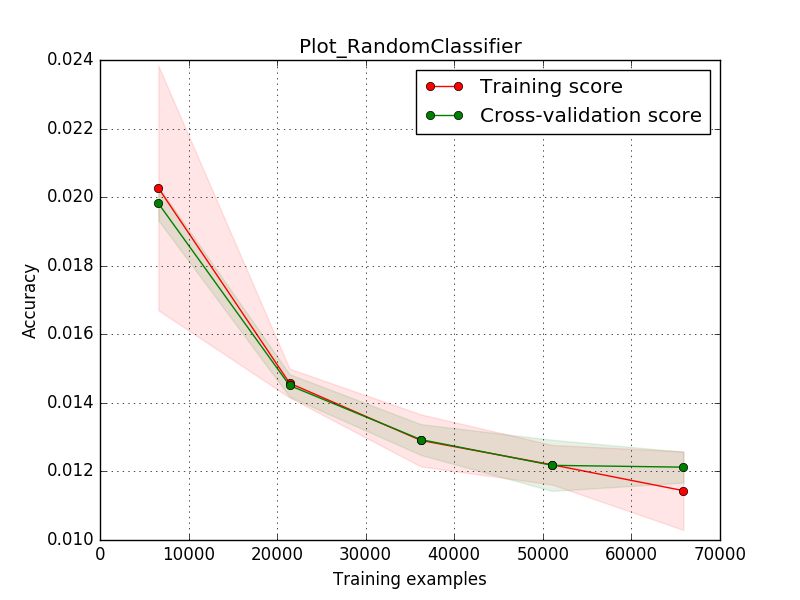
\includegraphics[width=0.6\textwidth]{Figures/Plot_RandomClassifier}
\decoRule
\caption[Random Baseline learning curve]{Random Baseline learning curve}
\label{fig:randombaseline}
\end{figure}

\noindent In Table~\ref{tab:baselinerandom} and Table~\ref{tab:baselinepositive} the scores are listed. The binary precision of Table~\ref{tab:baselinepositive} would give a divison by zero. If that is the case, the score is set to $0.0$. Both F-scores in both baselines are low. The random algorithm is terrible at classification. The closer to $0$ the F-score is, the less well the algorithm performs. The tables also list the amount of samples used, aswell as the binary classification. This is done to show how many samples were used in the test. The amount of positive and negative training samples is also shown.

\begin{table}[H]
\begin{minipage}{0.5\textwidth}
\caption{Baseline Random classifier (uniform): Average.}
\label{tab:baselinerandom}
\centering
\begin{tabular}{l r}
\toprule
Multi-class F-score & 0.0162 \\
Multi-class Precision & 0.1205 \\
Multi-class Recall & 0.0096 \\
\midrule
Binary F-score & 0.4653 \\
Binary Precision & 0.3592 \\
Binary Recall & 0.6603 \\
\midrule
Total amount of samples & 231797.0 \\
False negative & 28278.0 \\
False positive & 98054.15 \\
True negative & 50492.85 \\
True positive & 54972.0 \\
\midrule
Positive training samples & 82159.0 \\
Negative training samples & 49638.0 \\
\midrule
Variance Multi-class F-score & 1.18e-07 \\
Variance Multi-class Precision & 8.33e-06 \\
Variance Multi-class Recall & 4.46e-08 \\
\midrule
Variance Binary F-score & 8.21e-07 \\
Variance Binary Precision & 5.00e-07 \\
Variance Binary Recall & 2.48e-06 \\
\bottomrule
\end{tabular}
\end{minipage}
\begin{minipage}{0.5\textwidth}
\caption{Baseline Random classifier (All negative): Average.}
\label{tab:baselinepositive}
\centering
\begin{tabular}{l r}
\toprule
Multi-class F-score & 0.0287 \\
Multi-class Precision & 0.1104 \\
Multi-class Recall & 0.0183 \\
\midrule
Binary F-score & 0.0 \\
Binary Precision & 0.0 \\
Binary Recall & 0.0 \\
\midrule
Total amount of samples & 231797.0 \\
False negative & 83250.0 \\
False positive & 0.0 \\
True negative & 148547.0 \\
True positive & 0.0 \\
\midrule
Positive training samples & 0.0 \\
Negative training samples & 49638.0 \\
\midrule
Variance Multi-class F-score & 3.41e-07 \\
Variance Multi-class Precision & 4.51e-06 \\
Variance Multi-class Recall & 1.14e-07 \\
\midrule
Variance Binary F-score & 0.0 \\
Variance Binary Precision & 0.0 \\
Variance Binary Recall & 0.0 \\
\bottomrule
\end{tabular}
\end{minipage}
\end{table}

\section{K-nearest Neighbors}
K-nearest Neighbors as seen in Section~\ref{algorithm:knn} is a very promising algorithm for intrusion detection. $k$ was chosen at the default value of $5$.  However, different experiments have been done to compare the effect of $k$ on the perofrmance of the machine learning algorithm. The default distance metric that was used, is the Manhattan distance. In a realistic data-set, the malicious data is skewed. For this reason, the solution proposed in Section~\ref{knn:sol} was used. The first experiment that was done, was to construct the learning curve as seen in Figure~\ref{fig:knnlearn1}. \\
\\
Since KNN uses the $k$-closest neighbors and their distance to the to-be-predicted data point, it is normal that the training score is $1.0$. This is because the training score is calculated by feeding the training data to the machine learning algorithm to test it. The closest point to any training data point is that data point itself. This means that the algorithm will predict the same class. Overfitting is unlikely. In that case, the training score is expected to be high, but the cross-validation score should go down. It can be seen that the algorithm converges to an accuracy of about 86\%, but the algorithm shows a general trend to improve the accuracy when more training data is used. Underfitting is also unlikely because of this trend. 

 \begin{figure}[H]
\centering
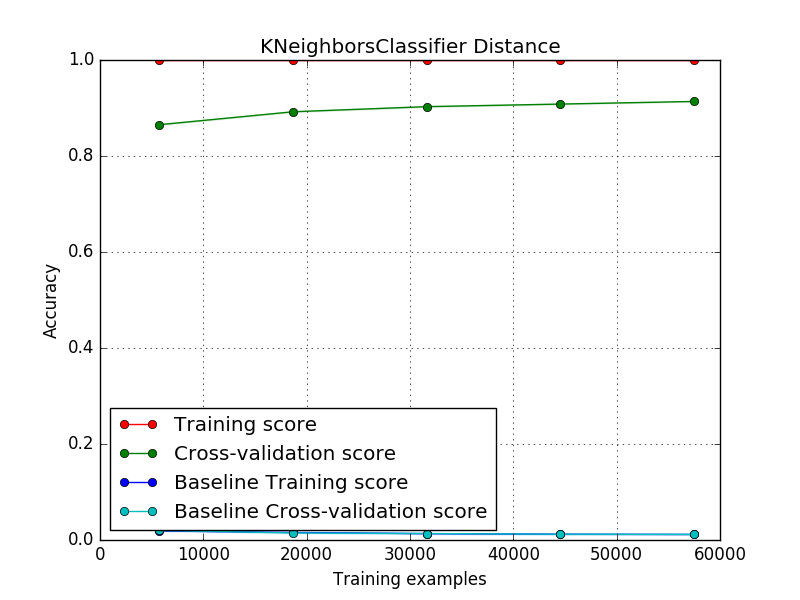
\includegraphics[width=0.6\textwidth]{Figures/KNeighborsClassifier_Distance}
\decoRule
\caption[Learning Curve for K-Nearest Neighbors]{Learning Curve for K-Nearest Neighbors}
\label{fig:knnlearn1}
\end{figure}

\noindent The first experiment using the F-score that has been done was a validation within the CTU dataset. This is shown in Table~\ref{tab:knn:ctu}. The experiment was done with all three feature sets. The algorithm was trained using $\sim80000$ samples with about as much malicious and non-malicious data. First the general results are discussed. Afterwards the different feature sets are discussed.\\
\\
The variance on both F-scores are very low, which means that the average result is statistically relevant. The binary F-score is $\sim0.9500$ is quite high. This means that the algorithm is able to distinguish between malicious and non-malicious data. The multi-class F-score is lower, which means the algorithm does make more mistakes concerning the exact classification. Together this means that the malicious data is grouped together, but the actual classes within the malicious data are less distinguishable. \\
\\
The effect of using the country of origin does not seem to have a lot of impact on the results. This could be due to the fact that the data belongs to a data set which contains data from mosty the same country. Using TCP flags does increase the performance immensely.  This means that the different classes do become more distinguisable when more data, and more specifically the TCP flags, are used. KNN uses the $k$-closest neighbors and their distance to the to-be-predicted data point. Because of the high binary and multi-class F-score, it can be said that most classes and more specifically, the malicious and non-malicious samples are grouped together. If different samples weren't grouped together, then the $k$-closest neighbors would be of different classes, and the F-score would be much lower.

\begin{table}[H]
\caption{K-Nearest Neighbors: comparing different feature sets: CTU-dataset}
\label{tab:knn:ctu}
\centering
\begin{tabular}{l c c r}
\toprule
Feature set & Standard & TCP & Country \\
\midrule
Multi-class F-score & 0.6153 & 0.8476 & 0.6149 \\
Multi-class Precision & 0.6820 & 0.8527 & 0.6863 \\
Multi-class Recall & 0.6280 & 0.8482 & 0.6278 \\
\midrule
Binary F-score & 0.9500 & 0.9857 & 0.9499\\
Binary Precision & 0.9204 & 0.9797 & 0.9202 \\
Binary Recall & 0.9816 & 0.9918 & 0.9816\\
\midrule
Total amount of samples & 195519.0 & 195519.0 & 195519.0 \\
False negative & 1048.0 & 466.5 & 1049.0 \\
False positive & 4830.0 & 1169.2 & 4841.0 \\
True negative & 133798.0 & 137458.8 & 133787.0 \\
True positive & 55843.0 & 56424.5 & 55842.0 \\
\midrule
Positive training samples & 35363.0 & 35363.0 & 35363.0\\
Negative training samples & 49638.0 & 49638.0 & 49638.0\\
\midrule
Variance Multi-class F-score & 1.23e-32 & 1.23e-32 & 1.23e-32 \\
Variance Multi-class Precision & 0.0 & 1.23e-32 & 1.23e-32 \\
Variance Multi-class Recall & 1.23e-32 & 0.0 & 1.23e-32 \\
\midrule
Variance Binary F-score & 0.0 & 1.23e-32 & 1.23e-32 \\
Variance Binary Precision & 0.0 & 0.0 & 4.93e-32 \\
Variance Binary Recall & 4.93e-32 & 0.0 & 1.23e-32 \\
\bottomrule
\end{tabular}
\end{table}

\noindent Table~\ref{tab:knn:cross} shows cross-dataset validation. It is interesting to see that the F-score is consistently higher than the F-scores from Table~\ref{tab:knn:ctu} . The positive samples consist of $30000$ samples from the SQL dataset and $35000$ samples from the CTU dataset. The amount of samples used for prediction consists of $50000$ samples from the SQL dataset and $\sim190000$ samples from the CTU dataset. \\
\\
The multi-class F-score is still high, which means that the algorithm is still able to correctly classify samples, even though data from different datasets are mixed. The high binary F-score means that the algorithm is able to correctly distinguish between malicious samples and non-malicious samples. The effect of the different feature sets is still the same in this experiment.  

\begin{table}[H]
\caption{K-Nearest Neighbors: comparing different feature sets: Cross-dataset}
\label{tab:knn:cross}
\centering
\begin{tabular}{l c c r}
\toprule
Feature set & Standard & TCP & Country \\
\midrule
Multi-class F-score & 0.7571 & 0.8798 & 0.7616 \\
Multi-class Precision & 0.7768 & 0.8839 & 0.7784 \\
Multi-class Recall & 0.7628 & 0.8803 & 0.7693 \\
\midrule
Binary F-score & 0.9631 & 0.9924 & 0.9713\\
Binary Precision & 0.9543 & 0.9892 & 0.9544 \\
Binary Recall & 0.9720 & 0.9956 & 0.9889\\
\midrule
Total amount of samples & 246467.0 & 246467.0 & 246467.0 \\
False negative & 3015.1 & 474.5 & 1200.6 \\
False positive & 5013.9 & 1172.2 & 5083.8 \\
True negative & 133614.1 & 137455.8 & 133544.2 \\
True positive & 104823.9 & 107364.5 & 106638.4 \\
\midrule
Positive training samples & 65363.0 & 65363.0 & 65363.0\\
Negative training samples & 49638.0 & 49638.0 & 49638.0\\
\midrule
Variance Multi-class F-score & 2.23e-08 & 1.20e-09 & 7.29e-07 \\
Variance Multi-class Precision & 4.99e-09 & 1.39e-09 & 7.62e-07 \\
Variance Multi-class Recall & 4.43e-08 & 5.77e-10 & 8.90e-07  \\
\midrule
Variance Binary F-score & 3.76e-08 & 5.20e-12 & 7.79e-09 \\
Variance Binary Precision & 1.35e-08 & 2.35e-15 & 1.33e-08 \\
Variance Binary Recall & 1.65e-07 & 2.06e-11 & 2.63e-08 \\
\bottomrule
\end{tabular}
\end{table}

\noindent During previous experiments, the standard feature set was used to find out how KNN performs and how the different feature sets weight in on the performance. In Table~\ref{tab:knn:k}, experiments were done using different values for $k$, the chosen values were $3$, $5$ and $7$. The results show that both $k=3$ and $k=7$ perform better than $k=5$. \\
\\
In order to be absolutly certain that no mistakes happened, the entire experiment (all 10 runs) was done again twice. The results remained the same. From this, it can be concluded that $k=5$ is a local minimum for the performance in relation to $k$. It can also be concluded that the actual value of $k$ needs to be determined experimentally when such a system would be set up in a data center since both $k=3$ and $k=7$ perform the same.  

\begin{table}[H]
\caption{K-Nearest Neighbors: comparing different values of K: Cross-dataset}
\label{tab:knn:k}
\centering
\begin{tabular}{l c c r}
\toprule
K & 3 & 5 & 7 \\
\midrule
Multi-class F-score & 0.8783 & 0.7571 & 0.8807 \\
Multi-class Precision & 0.8831 & 0.7768 & 0.8846 \\
Multi-class Recall & 0.8778 & 0.7628 & 0.8819 \\
\midrule
Binary F-score & 0.9924 & 0.9631 & 0.9926\\
Binary Precision & 0.9892 & 0.9543 & 0.9897 \\
Binary Recall & 0.9956 & 0.9720 & 0.9956\\
\midrule
Total amount of samples & 246467.0 & 246467.0 & 246467.0 \\
False negative & 474.5 & 3015.1 & 474.5 \\
False positive & 1172.2 & 5013.9 & 1117.4 \\
True negative & 137455.8 & 133614.1 & 137510.6 \\
True positive & 107364.5 & 104823.9 & 107364.5\\
\midrule
Positive training samples & 65363.0 & 65363.0 & 65363.0\\
Negative training samples & 49638.0 & 49638.0 & 49638.0\\
\midrule
Variance Multi-class F-score & 1.18e-09 & 2.23e-08 & 3.96e-10 \\
Variance Multi-class Precision & 8.69e-10 & 4.99e-09 & 5.43e-10 \\
Variance Multi-class Recall & 5.48e-10 & 4.43e-08 & 1.90e-10 \\
\midrule
Variance Binary F-score & 3.23e-11 & 3.76e-08 & 5.19e-12 \\
Variance Binary Precision & 1.47e-14 & 1.35e-08 & 1.30e-10 \\
Variance Binary Recall & 1.28e-10 & 1.65e-07 & 3.09e-11 \\
\bottomrule
\end{tabular}
\end{table}

\noindent Different experiments were also done to compare the effect of different distance metrics on the performance. The metrics that were used were the Manhattan distance, the Euclidean distance, the Chebyshev distance and the Canberra distance. These distances were introduced in Section~\ref{distancemetric}. The results of these experiments are shown in Table~\ref{tab:knn:dis}. \\
\\
The Manhattan distance performed the least. The Euclidean distance and the Chebyshev distance performed the same. The Canberra distance which is a weighted Manhattan distance has the best performance when looking at multi-class classification. The fact that the Canberra distance performs good and the Manhattan distance does not can be due to the fact that the Canberra distance is weighted. This means that the different features are not on scale which is indeed the case. \\
\\
The Canberra distance, however, is not the best when looking at the binary classification. Both the Euclidean distance and the Chebyshev distance perform better. Chebyshev works using the $max$ distanc between the features from two samples. In the Canberra metric, each feature has the same "importance". This could be the reason that Chebyshev works better for binary classification. Not every feature has the same importance. Chebyshev only uses the $max$ distance which most likely belongs to a feature which is more important for binary classification.\\
\\
It can be concluded that depending on the features that are chosen, different distance metrics need to be used. This means that when new features are added, new experiments should be done to find out which distance metric works the best.

\begin{table}[H]
\caption{K-Nearest Neighbors: comparing different distance metrics: Cross-dataset}
\label{tab:knn:dis}
\centering
\begin{tabular}{l c c c r}
\toprule
Distance metric & Manhattan & Euclidean & Chebyshev & Canberra \\
\midrule
Multi-class F-score & 0.7571 & 0.8772 & 0.8754 & 0.9151\\
Multi-class Precision & 0.7768 & 0.8814 & 0.8796 & 0.9216\\
Multi-class Recall & 0.7628 & 0.8778 & 0.8761 & 0.9122\\
\midrule
Binary F-score & 0.9631 & 0.9917 & 0.9912 & 0.9768\\
Binary Precision & 0.9543 & 0.9882 & 0.9874 & 0.9594 \\
Binary Recall & 0.9720 & 0.9951 & 0.9950 & 0.9950 \\
\midrule
Total amount of samples & 246467.0 & 246467.0 & 246467.0 & 539.2\\
False negative & 3015.1 & 528.4 & 539.2 & 4540.7 \\
False positive & 5013.9 & 1281.4 & 1369.2 & 4540.7 \\
True negative & 133614.1 & 137346.6 & 137258.8 & 134087.3 \\
True positive & 104823.9 & 107310.6 & 107299.9 & 107299.8\\
\midrule
Positive training samples & 65363.0 & 65363.0 & 65363.0 & 65363.0 \\
Negative training samples & 49638.0 & 49638.0 & 49638.0 & 49638.0\\
\midrule
Variance Multi-class F-score & 2.23e-08 & 3.63e-10 & 1.98e-09 & 1.56e-09\\
Variance Multi-class Precision & 4.99e-09 & 6.78e-10 & 2.73e-09 & 1.25e-09\\
Variance Multi-class Recall & 4.43e-08 & 2.09e-10 & 1.41e-09 &  1.49e-09\\
\midrule
Variance Binary F-score & 3.76e-08 & 1.43e-10 & 3.95e-11 & 1.94e-09\\
Variance Binary Precision & 1.35e-08 & 7.70e-14 & 6.93e-11 & 6.49e-10\\
Variance Binary Recall & 1.65e-07 & 5.68e-10 & 9.37e-11 & 5.38e-09\\
\bottomrule
\end{tabular}
\end{table}

\noindent As a final step, KNN was evaluated using a real-life unlabeled dataset. This was done using the Cegeka and EDM dataset. In Table~\ref{tab:knn:cegeka}, the results can be seen. The algorithm was tested on $\sim11000000$ samples. From these samples around $10000$ were from the EDM dataset. The others are from the Cegeka dataset. The algorithm does peform quite well with an F-score of $0.76$. 

\begin{table}[H]
\caption{K-Nearest Neighbors: real-world data}
\label{tab:knn:cegeka}
\centering
\begin{tabular}{l  r}
\toprule
F-score & 0.7633\\
\midrule
Total amount of samples & 11072646 \\
False negative &  8905 \\
False positive & 4164 \\
True negative &  11038482 \\
True positive & 21095 \\
\bottomrule
\end{tabular}
\end{table}

\newpage
\section{Decision Tree Classifier}

Decision tree classifiers which are seen in Section~\ref{decisiontree} were thought of as not very promising since they work on a simple principle. The results do show that the algorithm is quite good at intrusion detection. The learning curve, shown in Figure~\ref{fig:tree} shows that the training score and the cross-validation score do converge towards eachother. However, they converge quite slowly. This means that the decision tree classifier exhibits high variance. Due to the fact that neither the training score or the cross-validation score suddenly drop, it can be concluded that there is no overfitting. 

 \begin{figure}[H]
\centering
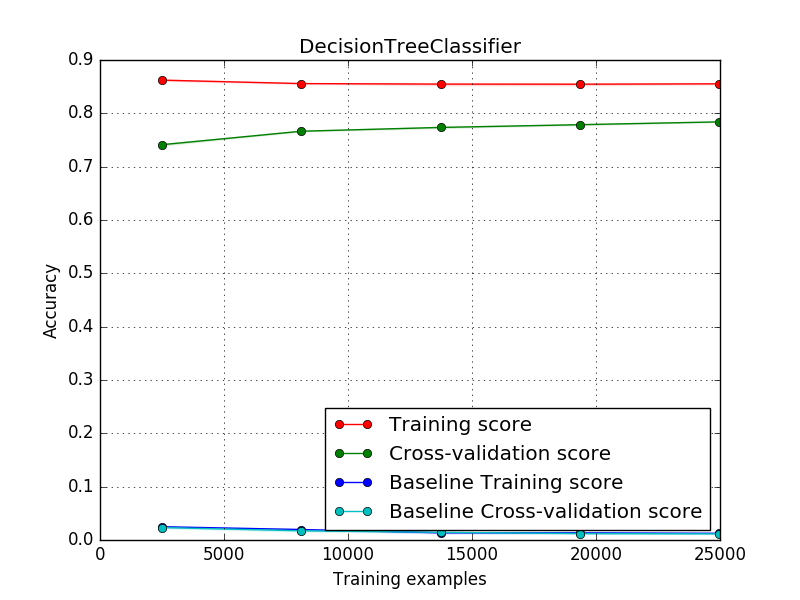
\includegraphics[width=0.6\textwidth]{Figures/Plot_DecisionTreeClassifier}
\decoRule
\caption[Learning Curve for Decision Tree Classifier]{Learning Curve for Decision Tree Classifier}
\label{fig:tree}
\end{figure}

\noindent Table~\ref{tab:tree:ctu} shows the results from the experiments that were done on the CTU-dataset. It also shows the comparison between the different feature sets. The F-score for multi-class classification is lower than the F-score from KNN. The fact that this score is lower could be due to the same reason as to why Decision tree classifiers didn't seem to be a promising algorithm. The tree is constructed using "decisions". These "decisions" could be to simple to be able to accuractly define a specific class. \\
\\
However, the high binary F-score shows that even though the decisions might not always lead to the correct classification, they do load to the correct decision of being malicious or non-malicious. The variance on the results is very small which means that the algorithm is stable and produces statistically relevant results. \\
\\
The different features perform is a similar way as they performed for KNN. Using the TCP flags increases the F-scores of the algorithm. This means that somewhere in the tree, a decision is made using these TCP flags and that this decision does help with correctly classifying the samples. The country feature set does not increment the performance. The results between the country feature set and the standard feature set only differ with just a few samples. The decision tree classifier is not able to use the country of origin at all. This does seem to follow the assumption that the dataset just does not contain enough different countries to allow the algorithm to make any decisions.

\begin{table}[H]
\caption{Decision Tree Classifier: comparing different feature sets: CTU-dataset}
\label{tab:tree:ctu}
\centering
\begin{tabular}{l c c r}
\toprule
Feature set & Standard & TCP & Country \\
\midrule
Multi-class F-score & 0.6001 & 0.6650 & 0.5999 \\
Multi-class Precision & 0.6571 & 0.7099 & 0.6570 \\
Multi-class Recall & 0.6008 & 0.6733 & 0.6007 \\
\midrule
Binary F-score & 0.9074 & 0.9511 & 0.9072 \\
Binary Precision & 0.8392 & 0.9175 & 0.8390 \\
Binary Recall & 0.9875 & 0.9873 & 0.9875 \\
\midrule
Total amount of samples & 195519.0 & 195519.0 & 195519.0 \\
False negative & 708.9  &  722.5 & 710.5 \\
False positive & 10762.7 & 5050.6 & 10778.9 \\
True negative & 127865.3 & 133577.4 & 127849.1  \\
True positive & 56182.1 & 56168.5  & 56180.5 \\
\midrule
Positive training samples & 25195.0 & 25195.0 & 25195.0\\
Negative training samples & 24806.0 & 24806.0 & 24806.0\\
\midrule
Variance Multi-class F-score & 1.44e-07 & 1.58e-07 & 2.44e-07 \\
Variance Multi-class Precision & 1.85e-07  &  1.92e-07 &  1.73e-07 \\
Variance Multi-class Recall &  1.76e-07 & 1.79e-07 &  2.59e-07  \\
\midrule
Variance Binary F-score & 2.92e-07  & 4.70e-08 & 5.80e-07  \\
Variance Binary Precision & 8.42e-07  &  9.15e-08  & 1.74e-06   \\
Variance Binary Recall & 8.92e-10 &  1.15e-07 & 1.56e-09 \\
\bottomrule
\end{tabular}
\end{table}

\noindent The results in Table~\ref{tab:tree:cross}, show the results of the cross-dataset evaluation which is used to evaluate the third step. Training is done using $19861$ non-malicious samples, $15000$ samples from the SQl dataset and $15000$ samples from the CTU dataset. The F-scores are higher than the F-scores from the CTU experiments. This means that the samples from the SQL dataset are more distinct and more easy to classify. It also means that the decision tree classifier is still able to correctly predict samples even though it is trained with multiple datasets. 

\begin{table}[H]
\caption{Decision Tree Classifier: comparing different feature sets: Cross-dataset}
\label{tab:tree:cross}
\centering
\begin{tabular}{l c c r}
\toprule
Feature set & Standard & TCP & Country \\
\midrule
Multi-class F-score & 0.7509 & 0.8042 & 0.7500 \\
Multi-class Precision & 0.7895 & 0.8307 & 0.7900 \\
Multi-class Recall & 0.7452 & 0.8057 & 0.7500 \\
\midrule
Binary F-score & 0.9413 & 0.9716 & 0.9400 \\
Binary Precision & 0.8946 & 0.9506 & 0.8900 \\
Binary Recall & 0.9932 & 0.9935 & 0.9900 \\
\midrule
Total amount of samples & 246467.0 & 246467.0 & 246467.0 \\
False negative & 729.7  &  700.9 & 723.9 \\
False positive & 12615.9 & 5567.7 & 12619.1 \\
True negative & 126012.1 &  133060.3 & 126008.9  \\
True positive & 107109.3 & 107138.1 & 107115.1 \\
\midrule
Positive training samples & 30140.0 & 30140.0 & 30140.0\\
Negative training samples & 19861.0 & 19861.0 & 19861.0\\
\midrule
Variance Multi-class F-score & 1.29e-07 & 1.93e-07 & 8.61e-08 \\
Variance Multi-class Precision & 1.98e-07  &  1.92e-07  &  1.08e-07 \\
Variance Multi-class Recall &  1.48e-07 &  3.21e-07 &  1.15e-07  \\
\midrule
Variance Binary F-score & 7.93e-08  & 2.05e-07 & 9.44e-08   \\
Variance Binary Precision & 2.56e-07  &  2.59e-07  & 3.19e-07    \\
Variance Binary Recall & 6.43e-09 &  2.50e-07  & 4.49e-09 \\
\bottomrule
\end{tabular}
\end{table}

\noindent As a final step, Decision tree classifiers were evaluated using a real-life unlabeled dataset. This was done using the Cegeka and EDM dataset. In Table~\ref{tab:knn:cegeka}, the results can be seen. The algorithm was tested on $\sim11000000$ samples. From these samples around $10000$ were from the EDM dataset. The others are from the Cegeka dataset. Surprisingly,  the algorithm generated a huge amount of false positives. This caused to algorithm to have a really low F-score. The reason that Decsion tree classifiers do not work well on real-world unlabeled data is probably because it is too fixated on the training data. The other evaluation tests got good results since the algorithm could work well on data that belonged to the same dataset. The decisions that the Decision tree classifier makes expect to be fed data that is very similar as the training dataset. This was the case for the other evaluation data, but not for the data from Cegeka and EDM.

\begin{table}[H]
\caption{Decision tree classifiers: real-world data}
\label{tab:tree:cegeka}
\centering
\begin{tabular}{l  r}
\toprule
F-score & 0.0155\\
\midrule
Total amount of samples & 11072646 \\
False negative & 14280  \\
False positive & 3245349 \\
True negative & 7787297 \\
True positive & 25720  \\
\bottomrule
\end{tabular}
\end{table}



\newpage
\section{Naive Bayes}

Naive Bayes has been explained in Section~\ref{bayesalg}. The algorithm uses the Theorem of Bayes. Not every feature is independent, for example it could be that the source and destination port are connected. Due to this reason, the algorithm was not that promising. This also showed during the experiments. \\
\\
The first experiment created the learning curve as seen in Figure~\ref{fig:naiveBayes}. In the beginning, with just a few samples, the accuracy is higher than when more training samples are used. This is due to the distribution of labels. Some labels appear more than others. When only 500 samples are used for training, most of these samples belong to classes that appear the most. Due to the fact that there are not many training samples, the algorithm has a higher chance of only predicting the most popular classes. The distribution of labels is similar when more training samples are used, but due to the higher amount of training samples, the algorithm trains more, and accounts for more labels.\\
\\
It can also be seen that both the training score and cross-validation score converge very fast. This signifies high bias and means that there is no point in training with more samples. 
 \begin{figure}[H]
\centering
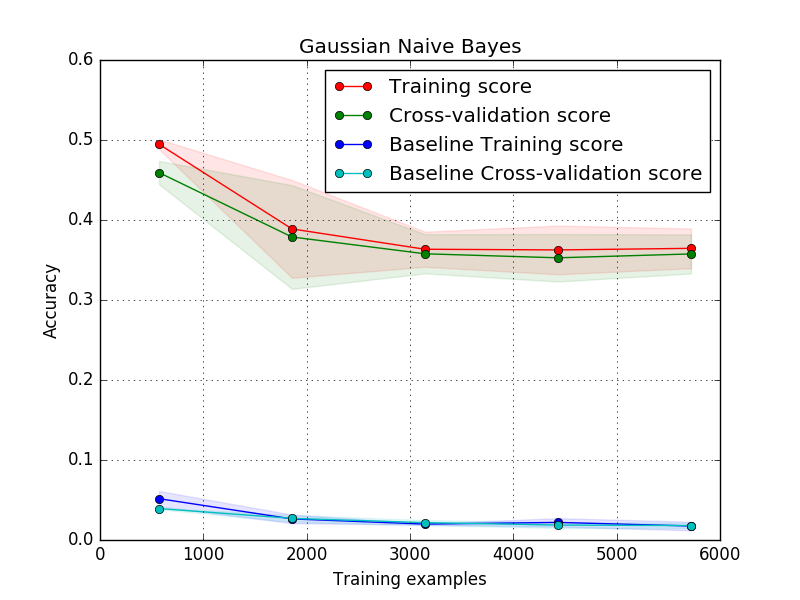
\includegraphics[width=0.6\textwidth]{Figures/Gaussian_Naive_Bayes}
\decoRule
\caption[Learning Curve for Gaussian Naive Bayes]{Learning Curve for Gaussian Naive Bayes}
\label{fig:naiveBayes}
\end{figure}

\noindent In Table~\ref{tab:bay:ctu}, the results from the CTU experiments can be seen. Immediatly two things can be seen. The scores are very low. The binary F-score is even lower than the F-score from the first baseline. The feature sets also have nearly no effect on the F-scores. The variance is also extremely small, which means these results are statistically relevant. This means that the Naive Bayes algorithm does not perform well at all. The fact that the feature sets have no effect can be contributed to the Naive assumption that is made. 	\\
\\
If the features are dependent on eachother, then the Naive assumption is completely wrong. The features extracted from flows are dependent on eachother. This can be due to the fact that packets on a network are always structured. An example would be that when the destination port is $80$, it can be expected that the protocol used is TCP. This signifies a dependence. 

\begin{table}[H]
\caption{Gaussian Naive Bayes: comparing different feature sets: CTU-dataset}
\label{tab:bay:ctu}
\centering
\begin{tabular}{l c c r}
\toprule
Feature set & Standard & TCP & Country \\
\midrule
Multi-class F-score & 0.3253 & 0.3253 & 0.3253 \\
Multi-class Precision & 0.2980 & 0.2980 & 0.2980 \\
Multi-class Recall & 0.4231 & 0.4232 & 0.4232 \\
\midrule
Binary F-score & 0.0146 & 0.0147 & 0.0147 \\
Binary Precision & 0.0179 & 0.0179 & 0.0179 \\
Binary Recall & 0.0123 & 0.0124 & 0.0124 \\
\midrule
Total amount of samples & 195519.0 & 195519.0 & 195519.0 \\
False negative & 56191.2  & 56186.0 & 56186.0 \\
False positive & 38393.0 & 38495.0 & 38495.0 \\
True negative & 100235.0 & 100133.0 & 100133.0 \\
True positive & 699.8 & 705.0 & 705.0 \\
\midrule
Positive training samples & 3545.0 & 3545.0 & 3545.0\\
Negative training samples & 4956.0 & 4956.0 & 4956.0\\
\midrule
Variance Multi-class F-score & 3.08e-33 & 3.08e-33 & 3.08e-33 \\
Variance Multi-class Precision & 0.0 &  0.0 & 0.0\\
Variance Multi-class Recall &  0.0 & 0.0 &  0.0   \\
\midrule
Variance Binary F-score & 0.0 &  0.0  & 0.0 \\
Variance Binary Precision & 1.20e-35 &  1.20e-35 & 1.20e-35  \\
Variance Binary Recall & 0.0 & 0.0 & 0.0 \\
\bottomrule
\end{tabular}
\end{table}

\noindent During the cross-dataset validation in Table~\ref{tab:bay:cross}, similar results can be seen. It can be noted that the binary F-score is higher and barely above the binary F-score from the first baseline. This means that even if the features are not independent, the algorithm can still see differences between SSH scans and normal traffic. Due to the fact that Bayes does not perform well at all, it has not been used in step four.

\begin{table}[H]
\caption{Gaussian Naive Bayes: comparing different feature sets: Cross-dataset}
\label{tab:bay:cross}
\centering
\begin{tabular}{l c c r}
\toprule
Feature set & Standard & TCP & Country \\
\midrule
Multi-class F-score & 0.3403 & 0.3398 & 0.3398 \\
Multi-class Precision & 0.3175 & 0.3170 & 0.3170 \\
Multi-class Recall & 0.4052 & 0.4047 & 0.4047 \\
\midrule
Binary F-score & 0.4990 & 0.4988 & 0.4986 \\
Binary Precision & 0.4854 & 0.4847 & 0.4843 \\
Binary Recall & 0.5134 & 0.5136 & 0.5137 \\
\midrule
Total amount of samples & 246467.0 & 246467.0 & 246467.0 \\
False negative & 52474.5  &  52452.9 & 52474.5 \\
False positive & 58695.1 & 58882.7 & 58695.1 \\
True negative & 79932.9 & 79745.3 & 79932.9  \\
True positive & 55364.5 & 55386.1 & 55364.5 \\
\midrule
Positive training samples & 6545.0 & 6545.0 & 6545.0\\
Negative training samples & 4956.0 & 4956.0 & 4956.0\\
\midrule
Variance Multi-class F-score & 3.26e-06 & 4.07e-06 & 4.92e-06\\
Variance Multi-class Precision & 3.31e-06 &  3.80e-06 & 4.52e-06 \\
Variance Multi-class Recall &  2.72e-06 & 3.90e-06 &  3.95e-06   \\
\midrule
Variance Binary F-score & 1.15e-06 & 1.31e-06 & 1.26e-06 \\
Variance Binary Precision & 5.09e-06 &  5.05e-06  & 3.07e-06   \\
Variance Binary Recall & 1.22e-06 &  8.18e-07 & 9.2e-07 \\
\bottomrule
\end{tabular}
\end{table}

\newpage
\section{Support Vector machines with Linear Kernel}

Support Vector Machines have also been tested. These have been explained in Section~\ref{svmalg}. First Support Vector Machines with a linear kernel have been tested. In the next section, Support Vector Machines with an RBF kernel has been used. \\
\\
The learning curve, shown in Figure~\ref{fig:svml}, is very irregular. It does not seem to follow a pattern at all. There is also a big standard deviation on the results. The accuracy almost matches the baseline in the worst case. Due to the irregular nature, it could lead to the conclusion that overfitting occurs since the cross-validation score drops. However, the training score also drops, which is not expected during overfitting. Underfitting could occur, but in that case it would be expected to see a slight increase in the accuracy instead on the extreme variance. 

 \begin{figure}[H]
\centering
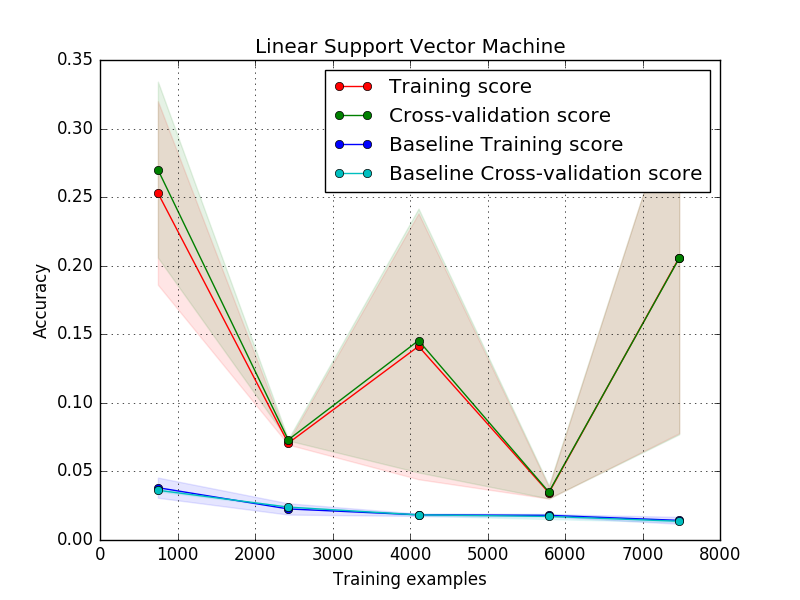
\includegraphics[width=0.6\textwidth]{Figures/Linear_Support_Vector_Machine}
\decoRule
\caption[Learning Curve for Linear Support Vector Machine]{Learning Curve for Linear Support Vector Machine}
\label{fig:svml}
\end{figure}

\noindent In Table~\ref{tab:linsvm:ctu}, the results from the experiments using the CTU dataset are shown. The first element that can be seen is the high variance. These mean that it becomes difficult to compare the results from the different feature sets. Furthermore, the F-scores are barely equal to the F-scores from the baseline. \\
\\
These scores and the variance can be explained due to the fact that intrusion detection cannot be solved using a linear classifier. Since there are a lot of features, it is difficult to plot them, so Figure~\ref{fig:linearvsNonLinearClassifier} from Section~\ref{linearclass} will be used. The linear classifier cannot group the different classes together. Every group created by the linear classifier still contains a lot of samples from other classes. This explains the low F-scores. Each time the experiment is done, the linear classifier is slightly different since it cannot find a way to correctly group the classes, this explains the high variance. 

\begin{table}[H]
\caption{Linear Kernel Support Vector Machine: comparing different feature sets: CTU-dataset}
\label{tab:linsvm:ctu}
\centering
\begin{tabular}{l c c r}
\toprule
Feature set & Standard & TCP & Country \\
\midrule
Multi-class F-score & 0.1015 & 0.0191 & 0.1883 \\
Multi-class Precision & 0.2091 & 0.0437 & 0.3218 \\
Multi-class Recall & 0.0918 & 0.0330 & 0.1621 \\
\midrule
Binary F-score & 0.4159 & 0.2267 & 0.4158 \\
Binary Precision & 0.2890 & 0.1470 & 0.2842 \\
Binary Recall & 0.7914 & 0.5007 & 0.7935 \\
\midrule
Total amount of samples & 195519.0 & 195519.0 & 195519.0 \\
False negative & 11866.5 & 28402.9 & 11747.6 \\
False positive & 90404.1 & 76436.5 & 87959.7 \\
True negative & 48223.9 & 62191.5 & 50668.3 \\
True positive & 45024.5 & 28488.1 & 45143.4 \\
\midrule
Positive training samples & 10069.0 & 10069.0 & 10069.0\\
Negative training samples & 9932.0 & 9932.0 & 9932.0\\
\midrule
Variance Multi-class F-score & 0.02 & 0.05 & 0.02020\\
Variance Multi-class Precision & 0.03 &  0.02 & 0.0279\\
Variance Multi-class Recall &  0.02 & 0.0001 &  0.0189   \\
\midrule
Variance Binary F-score & 0.05 &  0.05  & 0.0464 \\
Variance Binary Precision & 0.03 &  0.02 & 0.0233 \\
Variance Binary Recall & 0.15 & 0.25 & 0.1574 \\
\bottomrule
\end{tabular}
\end{table}

\noindent The cross-dataset experiments shown in Table~\ref{tab:linsvm:cross} have a lower variance. However, compared to other algorithms, the variance is still very high. The F-scores are overall a bit higher than the F-scores from the baseline, which means that the F-scores are not great at all. The results from this experiment are similar to the CTU experiment and the explanation of why the algorithm does not perform well is still supported due to the low scores and the high variance. Due to the fact that Support Vector Machines using a linear kernel do not perform well at all, it has not been used in step four.

\begin{table}[H]
\caption{Linear Kernel Support Vector Machine: comparing different feature sets: Cross-dataset}
\label{tab:linsvm:cross}
\centering
\begin{tabular}{l c c r}
\toprule
Feature set & Standard & TCP & Country \\
\midrule
Multi-class F-score & 0.2009 & 0.0369 & 0.2095 \\
Multi-class Precision & 0.3925 & 0.0533 & 0.4191 \\
Multi-class Recall & 0.1478 & 0.0497 & 0.1556 \\
\midrule
Binary F-score & 0.6041 & 0.4974 & 0.6390 \\
Binary Precision & 0.4952 & 0.4263 & 0.4703 \\
Binary Recall & 0.9183 & 0.6796 & 0.9971 \\
\midrule
Total amount of samples & 246467.0 & 246467.0 & 246467.0 \\
False negative & 8806.2  & 34551.5 & 314.2\\
False positive & 112296.5 & 89987.9 & 121331.3 \\
True negative & 26331.5 & 48640.1 & 517296.7 \\
True positive & 99032.8 & 73287.5 & 107524.8 \\
\midrule
Positive training samples & 10045.0 & 10045.0 & 10045.0\\
Negative training samples & 4956.0 & 4956.0 & 4956.0\\
\midrule
Variance Multi-class F-score & 0.0023 & 0.0027 & 0.0009\\
Variance Multi-class Precision & 0.0041 &  0.0053 & 0.0004\\
Variance Multi-class Recall &  0.0022 & 0.0049 &  0.0009   \\
\midrule
Variance Binary F-score & 0.0084 &  0.0309  & 0.0001 \\
Variance Binary Precision & 0.0084 &  0.0240 & 0.0002 \\
Variance Binary Recall & 0.0551 & 0.1003 & 1.1332e-06 \\
\bottomrule
\end{tabular}
\end{table}

\newpage
\section{Support Vector machines with RBF Kernel}

Support Vector Machines using a linear kernel did not work at all. They were barely better than the baseline. A conclusion was made that the classification cannot be made using linear classification. This can be verified by using a non-linear kernel. The kernel that was used, is the RBF kernel as seen in Section~\ref{kernels}. \\
\\
The learning curve is shown in Figure~\ref{fig:svmlearn}. Immediatly can be seen that the learning curve looks much better. The curve is regular. In this learning curve, it can be seen that there is a big gap between the cross-validation and training score. In underfitting, both the training and cross-validation score should be low. This cannot be seen in this learning curve. During overfitting, it would be expected that the training score is high since the model fits the training data very well, however the cross-validation score should be low and dropping. However, this also cannot be seen in this learning curve.

 \begin{figure}[H]
\centering
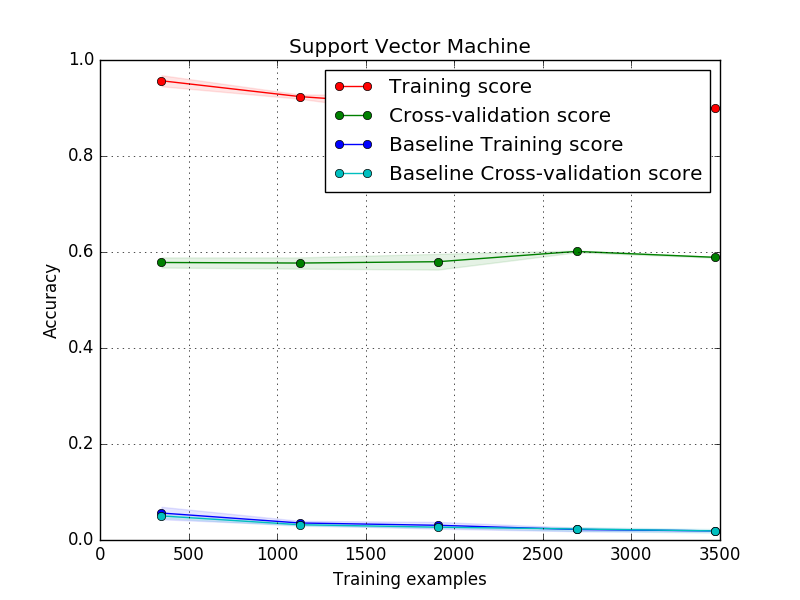
\includegraphics[width=0.6\textwidth]{Figures/Support_Vector_Machine}
\decoRule
\caption[Learning Curve for Support Vector Machine]{Learning Curve for Support Vector Machine}
\label{fig:svmlearn}
\end{figure}

\noindent The results from the CTU experiments are shown in Table~\ref{tab:svm:ctu}. The variance on both F-scores are very low which means we can compare the different F-scores. The multi-class F-scores are higher than the multi-class F-scores from the experiments with the linear kernel. This means that the exact classification happens better when using a non-linear kernel. This supports the idea that the classification cannot happen with a linear classifier. \\
\\
However, the binary F-score is extremely low. This is a result from using the RBF kernel. RBF kernels are also called Gaussian kernels. The kernel expects that training data follows a Gaussian distribution which is not the case for the training data from intrusion detection. The malicious and non-malicious samples do not follow a Gaussian distribution at all. When trying to classify samples using a Gaussian distribution, it cannot see the difference between malicious or non-malicious. However, the results from the multi-class F-score can still be compared to the multi-class F-score from the linear kernels. The multi-class F-score is still much higher than the multi-class F-score from the baseline. This means that the algorithm can still classify results better than randomly. The different feature sets also have little to no effect on the F-score, in case of the TCP feature set, it even lowers the F-score. 

\begin{table}[H]
\caption{RBF Kernel Support Vector Machine: comparing different feature sets: CTU-dataset}
\label{tab:svm:ctu}
\centering
\begin{tabular}{l c c r}
\toprule
Feature set & Standard & TCP & Country \\
\midrule
Multi-class F-score & 0.3641 & 0.3030 & 0.3643 \\
Multi-class Precision & 0.5124 & 0.5554 & 0.5167 \\
Multi-class Recall & 0.4037 & 0.3589 & 0.4062 \\
\midrule
Binary F-score & 0.0455 & 0.0282 & 0.0449 \\
Binary Precision & 0.0749 & 0.9987 & 0.0758 \\
Binary Recall & 0.0327 & 0.0143 & 0.0319 \\
\midrule
Total amount of samples & 195519.0 & 195519.0 & 195519.0 \\
False negative & 55029.0 & 56077.5 & 55075.0 \\
False positive & 22991.0 & 1.0 & 22115.0 \\
True negative & 115637.0 & 138627.0 & 116513.0 \\
True positive & 1862.0 & 813.5 & 1816.0\\
\midrule
Positive training samples & 2522.0 & 2522.0 & 2522.0\\
Negative training samples & 2479.0 & 2479.0 & 2479.0\\
\midrule
Variance Multi-class F-score & 3.08e-33 & 0.0 & 3.08e-33 \\
Variance Multi-class Precision & 0.0 & 1.23e-32 & 1.23e-32 \\
Variance Multi-class Recall & 1.23e-32 & 0.0 & 3.08e-33  \\
\midrule
Variance Binary F-score & 0.0 & 1.20e-35 & 4.81e-35 \\
Variance Binary Precision & 0.0 & 1.23e-32 & 0.0 \\
Variance Binary Recall & 4.81e-35 & 0.0 & 4.81e-35 \\
\bottomrule
\end{tabular}
\end{table}

\noindent The results from the cross-dataset validation are shown in Table~\ref{tab:svm:cross}. These results are much better. It seems that the SSH scans can
be detected better than the malware from the CTU dataset. The effect of using the TCP feature set and Country feature set is quite significant. This means that these feature do help the algorithm to correctly classifiy samples. However, this seems to only be the case for the SSH scans, not the samples from the CTU dataset. Due to the fact that Support Vector Machines using a RBF kernel do not perform well at all, it has not been used in step four.

\begin{table}[H]
\caption{RBF Kernel Support Vector Machine: comparing different feature sets: Cross-dataset}
\label{tab:svm:cross}
\centering
\begin{tabular}{l c c r}
\toprule
Feature set & Standard & TCP & Country \\
\midrule
Multi-class F-score & 0.3352 & 0.5761 & 0.5764 \\
Multi-class Precision & 0.6524 & 0.6944 & 0.6982 \\
Multi-class Recall & 0.4277 & 0.5979 & 0.5997 \\
\midrule
Binary F-score & 0.6740 & 0.6974 & 0.7001 \\
Binary Precision & 0.5083 & 0.7492 & 0.7567 \\
Binary Recall & 0.9999 & 0.6524 & 0.6514 \\
\midrule
Total amount of samples & 246467.0 & 246467.0 & 246467.0 \\
False negative & 10.8 & 37484.0 & 37584.4 \\
False positive & 104306.8 & 23541.0 & 22587.7 \\
True negative & 34321.2 & 115087.0 & 116040.3 \\
True positive & 107828.2 & 70355.0 & 70254.6 \\
\midrule
Positive training samples & 4522.0 & 4522.0 & 4522.0\\
Negative training samples & 2479.0 & 2479.0 & 2479.0\\
\midrule
Variance Multi-class F-score & 4.46e-08 & 3.92e-08 & 2.64e-07\\
Variance Multi-class Precision & 6.53e-06 & 3.30e-08 & 8.75e-08 \\
Variance Multi-class Recall & 2.16e-08 & 1.00e-07 & 6.01e-07  \\
\midrule
Variance Binary F-score & 5.71e-09 &  2.65e-07 & 1.42e-06\\
Variance Binary Precision & 6.50e-09 & 8.58e-08 & 1.96e-07 \\
Variance Binary Recall & 5.50e-09  & 4.76e-07 & 3.0685e-06 \\
\bottomrule
\end{tabular}
\end{table}

\newpage
\section{Neural network}

Neural networks were a promising algorithm. They were explained in Section~\ref{neuralnet}. Neural networks are quite complex and contain a lot of weights that need to be calculated during the training phase. Because of this, they require to be trained using a lot of data or they can be unstable and be in an underfitting phase. \\
\\
The learning curve can be seen in Figure~\ref{fig:neural}. The first thing that can be seen is that the training score and the cross-validation score are very close together. The scores are also dropping. Neural network requires a lot of training data. However, in the available datasets there is only a couple of thousand samples per malicious classification. The accuracy keeps dropping. This does not signify overfitting as the training score is also low. However, it does seem to be related to underfitting. During underfitting, it is expected that the training and cross-validation score drop to a local minimum and afterwards starts increases as the overfitting is resolved. However, there is not enough data to test when the overfitting is resolved.

 \begin{figure}[H]
\centering
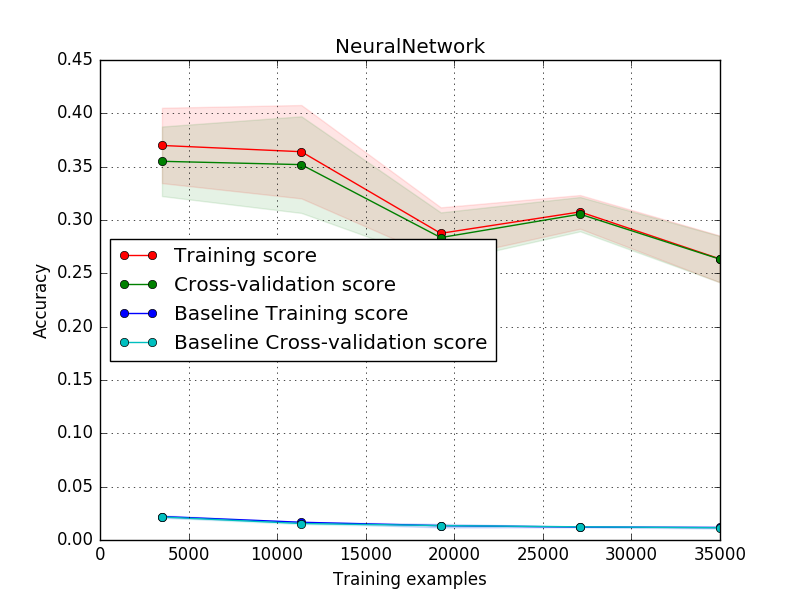
\includegraphics[width=0.6\textwidth]{Figures/NeuralNetwork}
\decoRule
\caption[Learning Curve for Neural Network]{Learning Curve for Neural Network}
\label{fig:neural}
\end{figure}

\noindent Even though the algorithm underfits, the experiments were still done. The results from the CTU dataset are shown in Table~\ref{tab:neural:ctu}. The Binary F-score is $0$ which means that the algorithm always classifies samples as non-malicious. The multi-class F-score is also quite low. This could be contributed to the underfitting. \\
\\
The biggest piece of evidence is the F-scores for the different feature sets. The multi-class F-scores for the TCP feature set and the Country feature set are much lower. These feature sets contain more features compared to the standard feature set. In a neural network, this means that more weights need to be calculated. This means that the overfitting should be worse when using more features. This is reflected in the F-scores for the TCP and Country feature set.

\begin{table}[H]
\caption{Neural Network: comparing different feature sets: CTU-dataset}
\label{tab:neural:ctu}
\centering
\begin{tabular}{l c c r}
\toprule
Feature set & Standard & TCP & Country \\
\midrule
Multi-class F-score & 0.2213 & 0.1322 & 0.1763 \\
Multi-class Precision & 0.2070 & 0.0854 & 0.1479 \\
Multi-class Recall & 0.3541 & 0.2922 & 0.3225 \\
\midrule
Binary F-score & 0.0 & 0.0 & 0.0 \\
Binary Precision & 0.0 & 0.0 & 0.0 \\
Binary Recall & 0.0 & 0.0 & 0.0 \\
\midrule
Total amount of samples & 195519.0 & 195519.0 & 195519.0 \\
False negative & 56891.0 & 56891.0 & 56891.0 \\
False positive & 0.0 & 0.0 & 0.0 \\
True negative & 138628.0 & 138628.0 & 138628.0 \\
True positive & 0.0 & 0.0 & 0.0 \\
\midrule
Positive training samples & 25195.0 & 25195.0 & 25195.0\\
Negative training samples & 24806.0 & 24806.0 & 24806.0\\
\midrule
Variance Multi-class F-score & 0.0019 & 7.70e-34 & 0.0029 \\
Variance Multi-class Precision & 0.0037 & 0.0 & 0.0059 \\
Variance Multi-class Recall & 0.0009 & 0.0 & 0.0013  \\
\midrule
Variance Binary F-score & 0.0 & 0.0 & 0.0 \\
Variance Binary Precision & 0.0 & 0.0 & 0.0 \\
Variance Binary Recall & 0.0 & 0.0 & 0.0 \\
\bottomrule
\end{tabular}
\end{table}

\noindent The results from the cross-dataset validation is shown in Table~\ref{tab:neural:cross}. The scores are yet again, quite low. The algorithm was trained using $20000$ samples from the SQL dataset, $25000$ malicious samples from the CTU dataset and $25000$ non-malicious samples from the CTU dataset. \\
\\
The binary F-score is much higher as compared to the CTU experiment. It has to be noted that the samples of the SQL dataset belong to a single class, SSH scans and that the malicious samples from the CTU dataset contain a lot of different malicious classes. This means that if the binary F-score is higher, the neural net does not underfit that much anymore on the classification between malicious and non-malicious. This is due to the SSH scan samples. This leads to the conclusion that the algorithm is should not underfit that much anymore when more than $20000$ samples are used for each class. \\
\\
It is also interesting that the multi-class F-score for the TCP feature set is much higher as compared to the other multi-class F-scores. This is also due to the samples from the SQL dataset. It seems that having these samples does indeed resolve a part of the underfitting, especially when the TCP flags are used. Even though more weights need to be calculated, it seems that the TCP flags help more than they cause underfitting. Due to the fact that Neural networks do not perform well and are underfitting, it has not been used in step four. 

\begin{table}[H]
\caption{Neural Network: comparing different feature sets: Cross-dataset}
\label{tab:neural:cross}
\centering
\begin{tabular}{l c c r}
\toprule
Feature set & Standard & TCP & Country \\
\midrule
Multi-class F-score & 0.1338 & 0.3679 & 0.1433 \\
Multi-class Precision & 0.0908 & 0.3328 & 0.0968 \\
Multi-class Recall & 0.2901 & 0.5021 & 0.2986 \\
\midrule
Binary F-score & 0.6128 & 0.5514 & 0.6056 \\
Binary Precision & 0.4426 & 0.5507 & 0.4437 \\
Binary Recall & 0.9970 & 0.5635 & 0.9641 \\
\midrule
Total amount of samples & 246467.0 & 246467.0 & 246467.0 \\
False negative & 316.9 & 47071.7 & 3867.5 \\
False positive & 135732.8 & 49578.2 & 130776.2 \\
True negative & 2895.2 & 89049.8 & 7851.8 \\
True positive & 107522.1 & 60767.3 & 103971.5 \\
\midrule
Positive training samples & 45195.0 & 45195.0 & 45195.0\\
Negative training samples & 24806.0 & 24806.0 & 24806.0\\
\midrule
Variance Multi-class F-score & 0.0006 & 0.0019 & 0.0013 \\
Variance Multi-class Precision & 0.0009 & 0.0028 & 0.0010 \\
Variance Multi-class Recall & 0.0003 & 0.0017 & 0.0009  \\
\midrule
Variance Binary F-score & 0.0001 & 0.0024 & 0.0006 \\
Variance Binary Precision & 0.0002 & 0.0039 & 0.0002 \\
Variance Binary Recall & 7.77e-05 & 0.0075 & 0.009 \\
\bottomrule
\end{tabular}
\end{table}

\newpage
\section{One-class Support Vector Machines}
\label{eval:oneclass}
One-class Support Vector Machines are the only unsupervised learning algorithms that have been used. They are explained in Section~\ref{oneclassSVM}. One-class Support Vector Machines only use a single class. The idea behind the algorithm was to perhaps use it as a preprocessor. If the algorithm would be able to correctly predict whether an element is malicious or non-malicious, it could be used before a supervised algorithm would be used. Afterwards, only the malicious samples would be fed to a supervised learning algorithm.\\
\\
Table~\ref{tab:one:cross} shows the results from different experiments that have been done. Yet again, it can be seen that using the TCP feature set does increase the performance. However, even with the TCP feature set, the binary F-score is barely as good as the baseline, a random classifier. Looking more closely, it can be seen that there are no true negatives in the TCP feature set experiment. However, there are false negatives. This means that the algorithm cannot be used at all for a preprocessing step.

\begin{table}[H]
\caption{One-class Support Vector Machine: comparing different feature sets: Cross-dataset}
\label{tab:one:cross}
\centering
\begin{tabular}{l c c r}
\toprule
Feature set & Standard & TCP & Country \\
\midrule
Binary F-score & 0.1275 & 0.4017 & 0.1557\\
Binary Precision & 0.1128 & 0.2911 & 0.1385 \\
Binary Recall & 0.1489 & 0.6480 & 0.1794\\
\midrule
Total amount of samples & 226467.0 & 226467.0 & 226467.0 \\
False negative & 74762.4 & 30912.0 & 72082.7 \\
False positive & 88162.5 & 138628.0 & 87260.7 \\
True negative & 50465.6 & 0.0 & 51367.3 \\
True positive & 13076.5 & 56927.0 & 15756.3 \\
\midrule
Positive training samples & 65000.0 & 65000.0 & 65000.0\\
Negative training samples & 0.0 & 0.0 & 0.0\\
\midrule
Variance Binary F-score & 0.0191 & 0.0006 & 0.0169 \\
Variance Binary Precision & 0.0125 &  0.0002 & 0.0116 \\
Variance Binary Recall & 0.0319 & 0.0024 & 0.0261 \\
\bottomrule
\end{tabular}
\end{table}
